
\documentclass{beamer}

\usepackage{animate}
\usepackage[round,authoryear]{natbib}

\newcommand{\Real}{\mathbb{R}}
\newcommand{\Int}{\mathbb{Z}}
\newcommand{\Nat}{\mathbb{N}}
\newcommand{\Complex}{\mathbb{C}}
\newcommand{\vect}[1]{\boldsymbol{#1}}

\usetheme{Boadilla}

\title{Understanding Asset Return Process}
\author{Jacques Nel}
\institute{York University}
\date{\today}

\begin{document}

\begin{frame}
\titlepage
\end{frame}

\begin{frame}
    \frametitle{Our problem}

    Develop a learning-to-rank investment strategy following the approach of
    \citep{song:1}

    \begin{enumerate}

        \item Given our universe of $n$ stocks, pick top $k$

        \item Train model on 2 years

        \item Test performance on 3rd year

        \item Report performance metrics:
            top-$k$ rank accuracy, average return, volatility, sharpe ratio, and max drawdown

        \item Compare with \texttt{S\&P500} index

    \end{enumerate}

\end{frame}

\begin{frame}

\frametitle{Achieving stationarity}

Neural network performance is dependent on stationarity of training data

Intuitively:

\begin{enumerate}

    \item Each example should look similar to the next, minus the dynamics we are trying to model
    \item Numerical performance implications

\end{enumerate}

In time series problems (including regression with ARIMA or GARCH), apply differencing scheme
to make data stationary.

Log-returns are the best choice in financial time series, ie., given a time series
$(s_t) \in \Real$, for $0< t\in\Int$:

$$
x_t = \log s_t - \log s_{t-1}
$$

\end{frame}

\begin{frame}

    \frametitle{Exploring our data}

    \begin{figure}
        \center
        \caption{Log-returns for 6 stocks}
    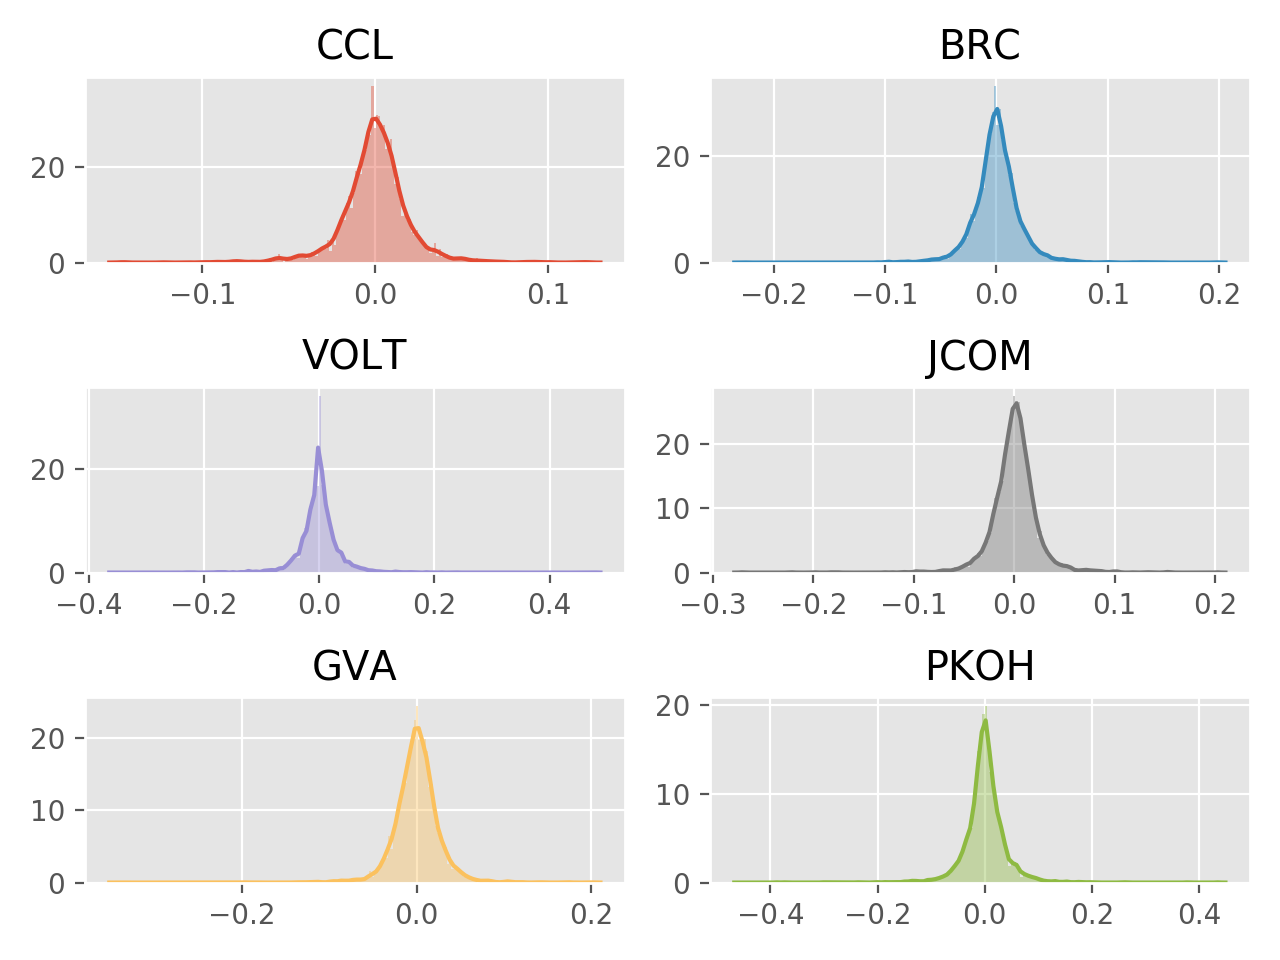
\includegraphics[scale=0.5]{log_ret}
\end{figure}

\end{frame}

\begin{frame}

Some observations:

\begin{enumerate}

    \item Log-returns maybe folow Laplace distribution

    \item Distributions have heavy tails

\end{enumerate}

\end{frame}

\begin{frame}

    \frametitle{Dilated Temporal Convolution Network (TCN) ie. WaveNet}

    \citep{wavenet:1} introduces high performance generative model for audio waveforms

    \begin{enumerate}

        \item Overcomes training problems of LSTMs, GRUs, and other RNN architectures

        \item No vanishing gradient

        \item Massive improvement in performance and memory usage
        
        \item Attains very long look-back (receptive field) using dilated convolutions

    \end{enumerate}

\end{frame}

\begin{frame}
    \frametitle{Dilated Temporal Convolution Network (TCN) ie. WaveNet}

    \begin{figure}
        \center
    \end{figure}

\end{frame}

\begin{frame}

    \frametitle{Generative Adverserial Network (GAN)}

    GANs are universal generators (analgolous to universal approximation theorem)

    \begin{figure}
        \center
        \includegraphics[scale=0.25]{gan}
    \end{figure}

\end{frame}

\begin{frame}

    \frametitle{Lambert W transformation}


Lambert's $W$ function is the inverse of $z=u\exp(u)$, ie. the function that satisfies

\begin{equation}
W(z)\exp(W(z))= z
\end{equation}

Let $U$ be a continous RV with cdf $F_U (u|\vect{\beta})$,
pdf $f_U(u|\vect{\beta})$, and parameter vector $\theta=(\vect{\beta},\delta)$, then

\begin{equation}
Z = U\exp\left(\frac{\delta}{2}U^2\right),\quad\delta\in\Real
\end{equation}

is a non-central, non-scaled heavy tail Lambert $W\times F_X$ RV with
parameter vector $\theta=(\vect{\beta},\delta)$, where $\delta$ is the
tail parameter.

\end{frame}

\begin{frame}

    \frametitle{Lambert W transformation}


For a continuous location-scale family RV $X~F_X(x|\vect{\beta})$ define a
location-scale heavy-tailed Lambert $W\times F_X$ RV

\begin{equation}\label{eq:trans}
Y=\left\lbrace U\exp\left(\frac{\delta}{2}U^2\right)\right\rbrace
\sigma_x+\mu_x,\quad\delta\in\Real
\end{equation}

Let $X~F_X(x|\vect{\beta})$ be continuous scale-family RV, with
standard deviation $\sigma_x$, let $U=X/\sigma_x$, then

\begin{equation}
Y=X\exp\left(\frac{\delta}{2}U^2\right),\quad\delta\in\Real,
\end{equation}

is a heavy-tailed Lambert $W\times F_X$ RV with parameter 
$\theta=(\vect{\beta},\delta)$.

Let $\tau:=(\mu_x(\vect{\beta}),\sigma_x(\vect{\beta}))$ define transformation
\cref{eq:trans}.

\end{frame}

\begin{frame}

    \frametitle{``Gaussianize'' heavy-tailed data}
The inverse transformation of \cref{eq:trans} is

\begin{equation}
W_\tau(Y):=W_\delta\left(\frac{Y-\mu_x}{\sigma_x}\right)\sigma_x
+\mu_x = U\sigma_x+\mu_x=X
\end{equation}

with

\begin{equation}
W_\delta(z,\delta) := \sgn(z)\left(\frac{W(\delta z^2)}{\delta}\right)^{1/2}.
\end{equation}

$W_\delta(z)$ is bijective for $\forall \delta>0$ and $\forall z\in\Real$.
\end{frame}

\begin{frame}

    \frametitle{MSE}



\end{frame}



\bibliography{cites}
\bibliographystyle{plainnat}
%\bibliographystyle{ieeetr}

\end{document}
